\section*{Kapitel 6 - Modelldiagnose}

\begin{multicols*}{3}

\tikzstyle{mybox} = [draw=black, fill=white, very thick,
    rectangle, rounded corners, inner sep=10pt, inner ysep=10pt]
\tikzstyle{fancytitle} =[fill=black, text=white, font=\bfseries]



%------------ Arten von Residuen ---------------
\begin{tikzpicture}
    \node [mybox] (box){%
        \begin{minipage}{0.3\textwidth}
        Gegeben sei das multiple lineare Regressionsmodell mit den üblichen Annahmen über $\beps$ und $\bX$.
        Aus Kapitel 2 wissen wir, dass $\V(\hbeps) = \sigma^2 \bQ$ und somit $\V(\hat{\eps_i}) = \sigma^2 q_{ii}$,
        wobei $q_{ii}$ das $i$-te Diagonalelement der Matrix $\bQ$ ist.

        Wir definieren \tc{standardisierte Residuen} als
        \begin{align*}
            r_i &= \frac{\hat{\eps_i}}{\sqrt{\hat{\sigma}^2 q_{ii}}}
        \end{align*}
        
        Das Problem an den standardisierten Residuen ist, dass bei der Schätzung
        von $\sigma^2$ die Residuen mit einbezogen werden. Dies führt zu einer
        Verzerrung der Residuen. Wir definieren daher zusätzlich
        \tc{studentisierte Residuen} als

        \begin{align*}
            r_i^* &= \frac{\hat{\eps_i}}{\sqrt{\hat{\sigma}_{(i)}^2 q_{ii}}}\\
            & = r_i \sqrt{\frac{n-p-1}{n-p-r_i^2}} \sim t_{n-p-1}
        \end{align*}
        wobei $\hat{\sigma}_{(i)}^2$ die Schätzung von $\sigma^2$ ist, die ohne die $i$-te
        Beobachtung berechnet wurde.
        Man kann zeigen, dass die studentisierten Residuen $t$-verteilt sind.

        Wir können 

    \end{minipage}
    };
%------------ Arten von Residuen Header ---------------------
\node[fill = black, text=white, font=\bfseries, right=10pt] at (box.north west) 
{Arten von Residuen};
\end{tikzpicture}

%------------ Durbin-Watson-Test ---------------
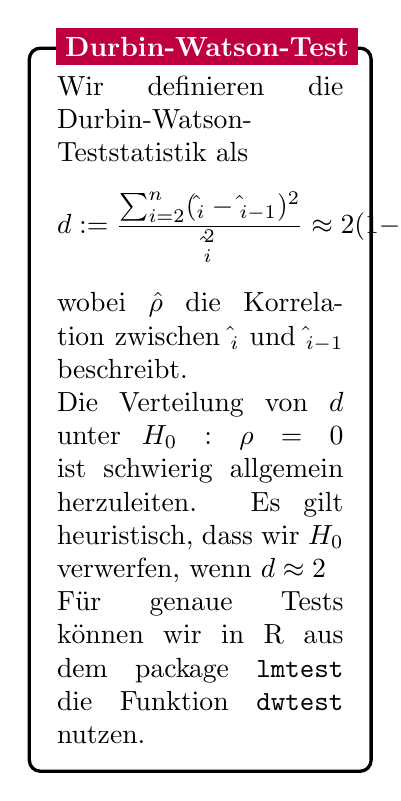
\begin{tikzpicture}
    \node [mybox] (box){%
        \begin{minipage}{0.3\textwidth}
        
        Wir definieren die \tc{Durbin-Watson-Teststatistik} als
        $$d := \frac{\sum_{i = 2}^{n} (\hat{\eps}_i - \hat{\eps}_{i-1})^2}{\sumin \hat{\eps}_i^2} \approx 2(1-\hat{\rho})$$
        wobei $\hat{\rho}$ die Korrelation zwischen $\hat{\eps}_i$ und $\hat{\eps}_{i-1}$ beschreibt.

        Die Verteilung von $d$ unter $H_0: \rho = 0$ ist schwierig allgemein herzuleiten.
        Es gilt heuristisch, dass wir $H_0$ verwerfen, wenn $d \approx 2$

        Für genaue Tests können wir in R aus dem package $\tt{lmtest}$ die Funktion $\tt{dwtest}$ nutzen.


    \end{minipage}
    };
%------------ Durbin-Watson-Test Header ---------------------
\node[fill = purple, text=white, font=\bfseries, right=10pt] at (box.north west) 
{Durbin-Watson-Test};
\end{tikzpicture}



%------------ Mögliche Probleme ---------------
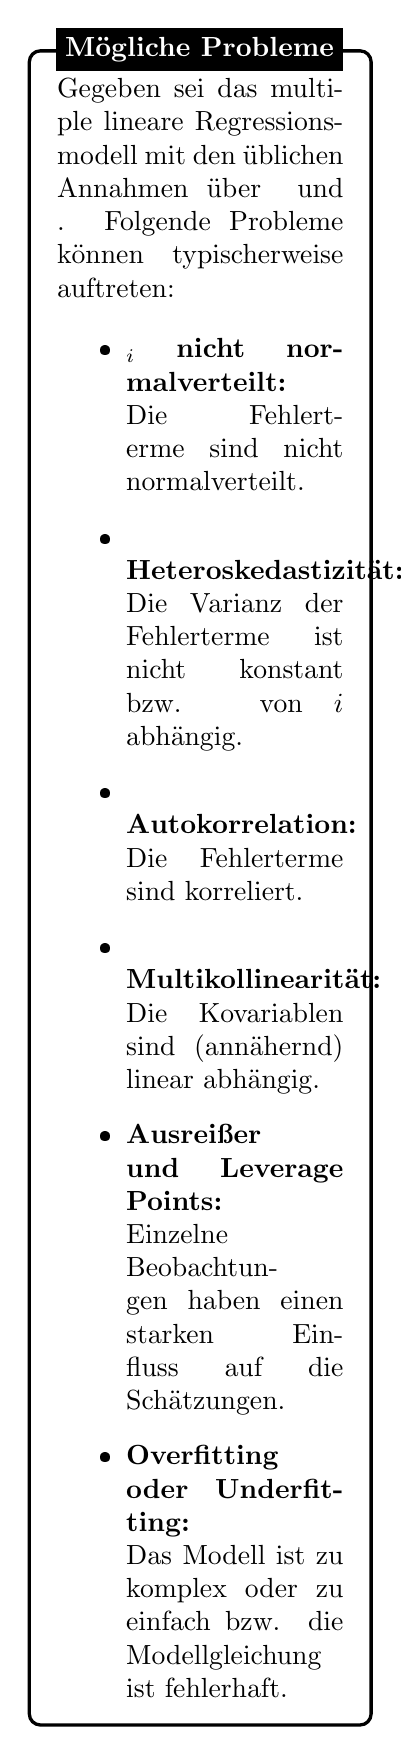
\begin{tikzpicture}
    \node [mybox] (box){%
        \begin{minipage}{0.3\textwidth}
        Gegeben sei das multiple lineare Regressionsmodell mit den üblichen Annahmen über $\beps$ und $\bX$.
        Folgende Probleme können typischerweise auftreten:

        \begin{itemize}
            \item \textbf{$\eps_i$ nicht normalverteilt:} \\
            Die Fehlerterme sind nicht normalverteilt.
            \item \textbf{Heteroskedastizität:} \\
            Die Varianz der Fehlerterme ist nicht konstant bzw. von $i$ abhängig.
            \item \textbf{Autokorrelation:} \\
            Die Fehlerterme sind korreliert.
            \item \textbf{Multikollinearität:} \\
            Die Kovariablen sind (annähernd) linear abhängig.
            \item \textbf{Ausreißer und Leverage Points:} \\
            Einzelne Beobachtungen haben einen starken Einfluss auf die Schätzungen.
            \item \textbf{Overfitting oder Underfitting:} \\
            Das Modell ist zu komplex oder zu einfach bzw. die Modellgleichung ist fehlerhaft.
        \end{itemize}

    \end{minipage}
    };
%------------ Mögliche Probleme Header ---------------------
\node[fill = black, text=white, font=\bfseries, right=10pt] at (box.north west) 
{Mögliche Probleme};
\end{tikzpicture}

%------------ Mögliche Probleme 1 ---------------
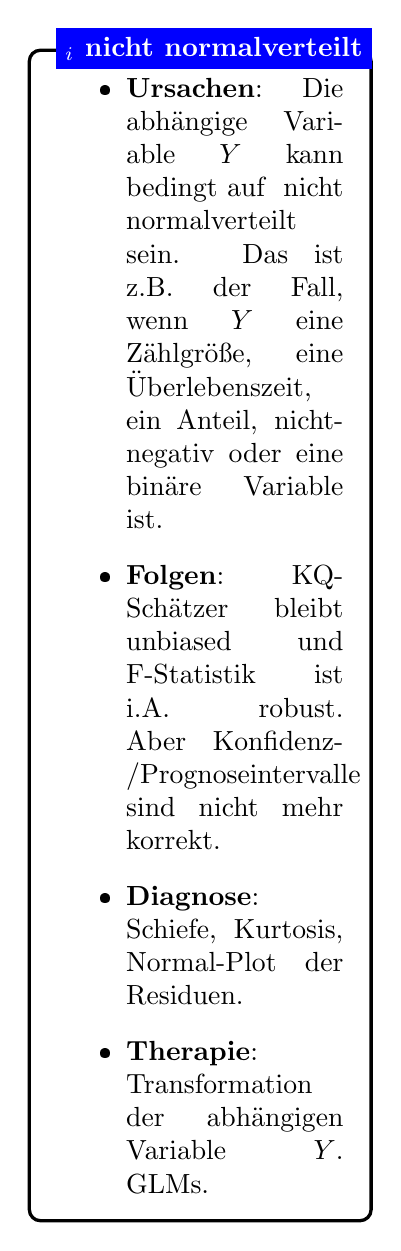
\begin{tikzpicture}
    \node [mybox] (box){%
        \begin{minipage}{0.3\textwidth}

        \begin{itemize}
            \item \textbf{Ursachen}: Die abhängige Variable $Y$ kann bedingt auf
            $\bx$ nicht normalverteilt sein. Das ist z.B. der Fall, wenn $Y$
            eine Zählgröße, eine Überlebenszeit, ein Anteil, nicht-negativ oder
            eine binäre Variable ist.
            \item \textbf{Folgen}: KQ-Schätzer bleibt unbiased und F-Statistik ist i.A.
            robust. Aber Konfidenz-/Prognoseintervalle sind nicht mehr korrekt.
            \item \textbf{Diagnose}: Schiefe, Kurtosis, Normal-Plot der Residuen.
            \item \textbf{Therapie}: Transformation der abhängigen Variable $Y$. GLMs.
        \end{itemize}

    \end{minipage}
    };
%------------ Mögliche Probleme 2 Header ---------------------
\node[fill = blue, text=white, font=\bfseries, right=10pt] at (box.north west) 
{$\eps_i$ nicht normalverteilt};
\end{tikzpicture}

%------------ Heteroskedastizität ---------------
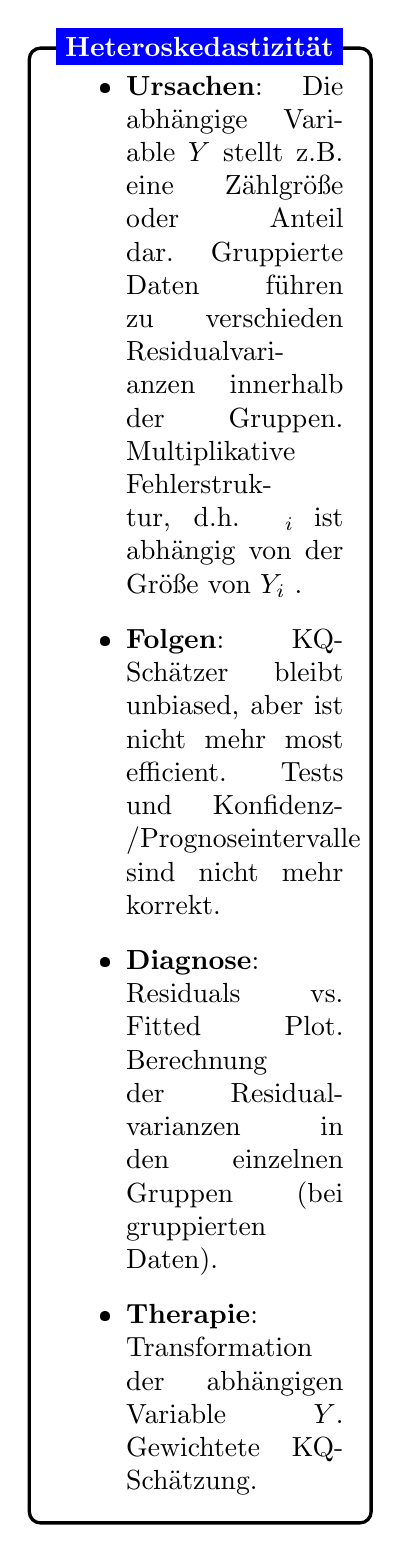
\begin{tikzpicture}
    \node [mybox] (box){%
        \begin{minipage}{0.3\textwidth}

        \begin{itemize}
            \item \textbf{Ursachen}: Die abhängige Variable $Y$ stellt z.B. eine
            Zählgröße oder Anteil dar. Gruppierte Daten führen zu verschieden
            Residualvarianzen innerhalb der Gruppen. Multiplikative
            Fehlerstruktur, d.h. $\ssd_i$ ist abhängig von der Größe von $Y_i$ .
            \item \textbf{Folgen}: KQ-Schätzer bleibt unbiased, aber ist nicht mehr most
            efficient. Tests und Konfidenz-/Prognoseintervalle sind nicht mehr
            korrekt.
            \item \textbf{Diagnose}: Residuals vs. Fitted Plot. Berechnung der
            Residualvarianzen in den einzelnen Gruppen (bei gruppierten Daten).
            \item \textbf{Therapie}: Transformation der abhängigen Variable $Y$.
            Gewichtete KQ-Schätzung.
        \end{itemize}

    \end{minipage}
    };
%------------ Heteroskedastizität Header ---------------------
\node[fill = blue, text=white, font=\bfseries, right=10pt] at (box.north west) 
{Heteroskedastizität};
\end{tikzpicture}


%------------ Autokorrelation ---------------
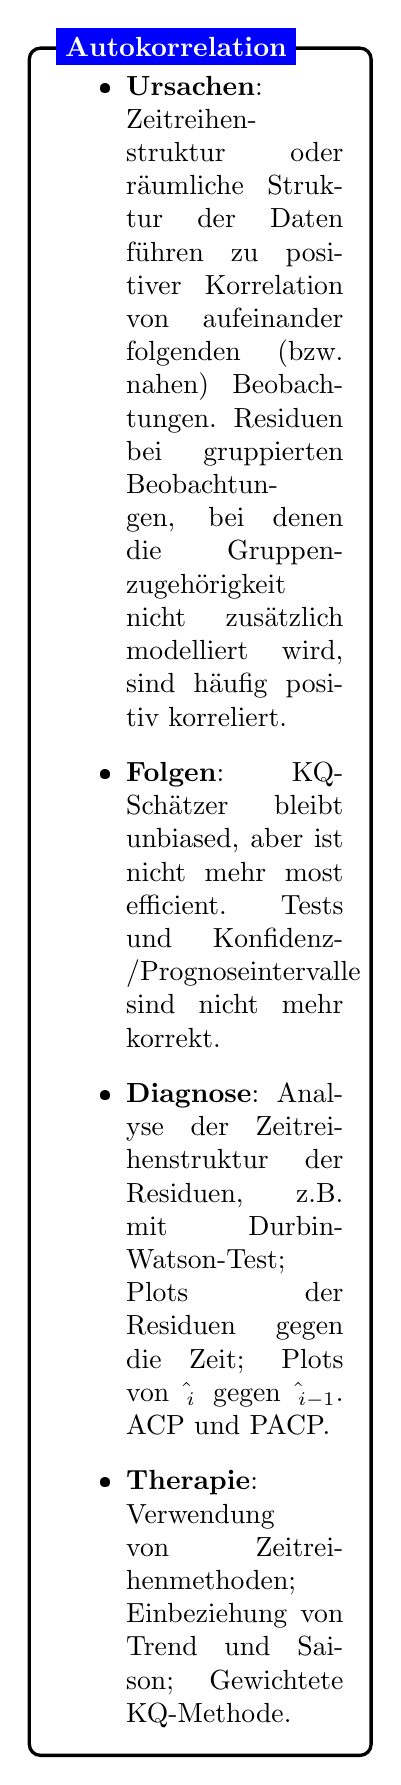
\begin{tikzpicture}
    \node [mybox] (box){%
        \begin{minipage}{0.3\textwidth}

        \begin{itemize}
            \item \textbf{Ursachen}: Zeitreihenstruktur oder räumliche Struktur
            der Daten führen zu positiver Korrelation von aufeinander folgenden
            (bzw. nahen) Beobachtungen. Residuen bei gruppierten Beobachtungen,
            bei denen die Gruppenzugehörigkeit nicht zusätzlich modelliert wird,
            sind häufig positiv korreliert.
            \item \textbf{Folgen}: KQ-Schätzer bleibt unbiased, aber ist nicht mehr most
            efficient. Tests und Konfidenz-/Prognoseintervalle sind nicht mehr
            korrekt.
            \item \textbf{Diagnose}: Analyse der Zeitreihenstruktur der
            Residuen, z.B. mit Durbin-Watson-Test; Plots der Residuen gegen die
            Zeit; Plots von $\hat{\eps}_i$ gegen $\hat{\eps}_{i-1}$. ACP und PACP.
            \item \textbf{Therapie}: Verwendung von Zeitreihenmethoden;
            Einbeziehung von Trend und Saison; Gewichtete KQ-Methode.

        \end{itemize}

    \end{minipage}
    };
%------------ Autokorrelation Header ---------------------
\node[fill = blue, text=white, font=\bfseries, right=10pt] at (box.north west) 
{Autokorrelation};
\end{tikzpicture}


%------------ Multikollinearität ---------------
\begin{tikzpicture}
    \node [mybox] (box){%
        \begin{minipage}{0.3\textwidth}

        \begin{itemize}
            \item \textbf{Ursachen}: Hohe Korrelation zwischen den Einflussgrößen; Ungünstiges
            Versuchs-Design; Codierung von diskreten Variablen.
            \item \textbf{Folgen}: Ungenauer KQ-Schätzer, häufig sogar mit falschem Vorzeichen. Aber
            Konfidenzintervalle sind korrekt (jedoch entsprechend sehr breit).
            \item \textbf{Diagnose}: Analyse der Matrix $\bX^\top \bX$ und der Korrelationsmatrix der
            metrischen Einflussgrößen.
            \begin{itemize}
                \item Konditionszahl von $\bX$: 
                $$\kappa(\bX) = \sqrt{\frac{\lambda_{max}(\bX^\top
                \bX)}{\lambda_{min}(\bX^\top \bX)}}$$
                $\kappa(\bX) \gg 1$ deutet auf Multikollinearität hin.
                \item Varianz Inflationsfaktor: $$\V(\hbe{j}) =
                \frac{\sigma^2}{(1-R_j^2) \sumin (x_{ij} - \overline{\bx_j})},$$
                wobei $R_j^2$ das Bestimmheitsmaß der Regression $\bX_j =
                \bX_{-j}\mathbf{\alpha} + \mathbf{\delta}$ ist. Wir definieren
                den \tc{Varianz Inflationsfaktor} als $$VIF_j =
                \frac{1}{1-R_j^2}.$$ Wenn $VIF_j = 1$, dann heißt das, dass
                $\bX_j$ orthogonal zu allen anderen Regressoren ist. Ein hohes
                $VIF_j$ deutet auf Multikollinearität hin. Als Heuristik wird
                oft $VIF_j > 10$ als kritisch angesehen.
                
            \end{itemize}
            \item \textbf{Therapie}: Zusammenfassen bzw. Weglassen von
            Einflussgrößen; Verwendung von anderen Schätzmethoden, z.B.:
            Ridge-Regression.
        \end{itemize}

    \end{minipage}
    };
%------------ Multikollinearität Header ---------------------
\node[fill = blue, text=white, font=\bfseries, right=10pt] at (box.north west) 
{Multikollinearität};
\end{tikzpicture}


%------------ Ausreißer und Leverage Points ---------------
\begin{tikzpicture}
    \node [mybox] (box){%
        \begin{minipage}{0.3\textwidth}
        Wir unterscheiden zwischen Ausreißern und High Leverage Points
        (einflußreiche Beobachtungen). Ein \tc{Ausreißer} ist eine Beobachtung,
        die in der abhängigen Variable $Y$ stark von den anderen Beobachtungen
        abweicht (i.d.R. hoher Störterm). Ein \tc{Leverage Point} ist eine
        Beobachtung, die in den unabhängigen Variablen $\bX$ stark von den
        anderen Beobachtungen abweicht.
        \begin{itemize}
            \item \textbf{Ursachen}: Falsche Erhebung; Beobachtung gehört
            nicht zur Grundgesamtheit; Besonderheiten bei einzelner
            Untersuchungseinheit.
            \item \textbf{Folgen}: High Leverage Points haben einen großen
            Einfluss auf $\hbbeta$. Ausreißer können zu erheblicher Verzerrung
            von $\hbbeta$ führen.
            \item \textbf{Diagnose}: Analyse der Diagonalelemente der Hat-Matrix
            $\bP$ zum Auffinden von high leverage points; Verschiedene Residuenplots
            zur Ausreißeranalyse; Influence-Statistiken.
            \item \textbf{Therapie}: Fehlerhafte Daten weglassen
            (Sensitivitätsanalyse); Robuste Regression; Gewichtete Regression.

        \end{itemize}

        Wir definieren \tc{Leverage} als
        \begin{align*}
            h_{ii} &= \bP_{ii} = \frac{\V(\hbY_i)}{\ssd} \\
            &=\bx_i^\top (\bX^\top \bX)^{-1} \bx_i = \lVert \bx_i \rVert^2_{(\bX^\top \bX)^{-1}}
        \end{align*}
        Optimalerweise gilt $h_{ii} = \frac{p'}{n}$ und 
        als Heuristik wird oft $h_{ii} > \frac{2p'}{n}$ als kritisch angesehen.\\
        \tc{!} Der Leverage kann nach Transformation auch als quadratischer
        Mahalanobis-Abstand zum Mittelpunkt interpretiert werden.
        
        Wir definieren \tc{Cook's Distanz} als
        \begin{align*}
            D_i &:= \frac{(\hbbeta_{-i} - \hbbeta)^\top (\bX^\top \bX)
            (\hbbeta_{-i} - \hbbeta)}{\hssd p'} \\
            &= \frac{(\hbY_{-i} - \hbY)^\top
            (\hbY_{-i} - \hbY)}{\hssd p'} \\
            &= \frac{r_i^2}{p'} \cdot \frac{h_{ii}}{1-h_{ii}}
        \end{align*}
        Als Heuristik wird oft verwendet, dass Beobachtungen mit $D_i > 0.5$
        auffällig sind und Beobachtungen mit $D_i > 1$ auf jeden Fall untersucht
        werden sollten.
    \end{minipage}
    };
%------------ Ausreißer und Leverage Points Header ---------------------
\node[fill = blue, text=white, font=\bfseries, right=10pt] at (box.north west) 
{Ausreißer und Leverage Points};
\end{tikzpicture}

%------------ Overfitting oder Underfitting ---------------
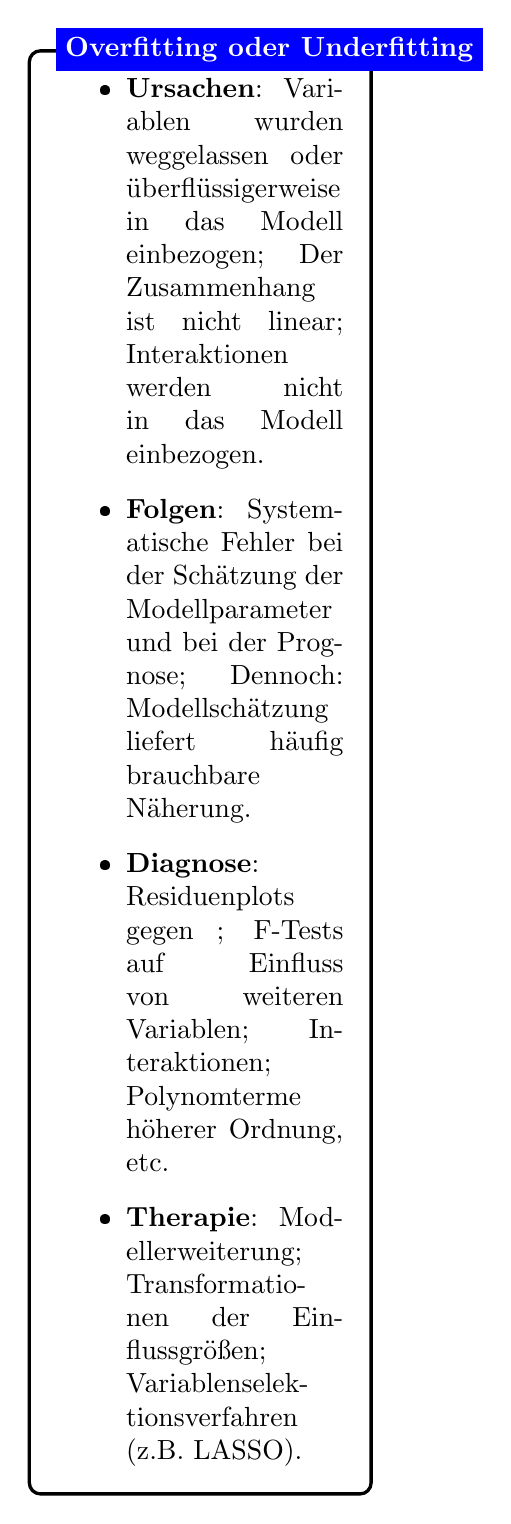
\begin{tikzpicture}
    \node [mybox] (box){%
        \begin{minipage}{0.3\textwidth}

        \begin{itemize}
            \item \textbf{Ursachen}: Variablen wurden weggelassen oder
            überflüssigerweise in das Modell einbezogen; Der Zusammenhang ist
            nicht linear; Interaktionen werden nicht in das Modell einbezogen.

            \item \textbf{Folgen}: Systematische Fehler bei der Schätzung der
            Modellparameter und bei der Prognose; Dennoch: Modellschätzung
            liefert häufig brauchbare Näherung.

            \item \textbf{Diagnose}: Residuenplots $\hbeps$ gegen $\hbY$;
            F-Tests auf Einfluss von weiteren Variablen; Interaktionen;
            Polynomterme höherer Ordnung, etc.

            \item \textbf{Therapie}: Modellerweiterung; Transformationen der
            Einflussgrößen; Variablenselektionsverfahren (z.B. LASSO).

        \end{itemize}

    \end{minipage}
    };
%------------ Overfitting oder Underfitting Header ---------------------
\node[fill = blue, text=white, font=\bfseries, right=10pt] at (box.north west) 
{Overfitting oder Underfitting};
\end{tikzpicture}



\end{multicols*}